%!TEX root = ../thesis.tex
\chapter{Introduction}
\label{ch:introduction}

%\epigraph{``As buds give rise by growth to fresh buds, and these, if vigorous, branch out and overtop on all sides many a feebler branch, so by generation I believe it has been with the great Tree of Life, which fills with its dead and broken branches the crust of the earth, and covers the surface with its ever-branching and beautiful ramifications.''}{Charles Darwin, 1872}

Charles Darwin's \emph{On the Origin of Species} contains a single figure, depicting the ancestry of species as a branching genealogical tree, or \emph{phylogeny} \cite{Darwin:1859uh} (see Figure \ref{fig:darwin_origin}).
Darwin argued that evolution was mediated by descent with modification; that is, the gradual change in heritable traits under the pressure of natural selection.
Since that time, the tree structure has been the dominant framework to understand, visualize, and communicate discoveries about evolution.
Indeed, an important aim of evolutionary biology has been expanding the \emph{universal tree of life}, the set of evolutionary relationships among all extant and extinct organisms on Earth \cite{Bowler:2003uz}.

Traditionally, evolutionary relationships were established on the basis of phenotype, i.e. the observable traits of each organism.
With the advent of molecular models of evolution and rapidly increasing genomic sequence data, the genotype has supplanted phenotype as the primary focus of evolutionary studies.
Molecular phylogenetics has become established as the standard tool for inferring phylogenetic relationships.
However, a phylogenetic tree is accurate only if the Darwinian model of descent with modification is the sole process driving evolution.
It has long been recognized that there exist alternative evolutionary processes that can allow organisms to directly exchange genetic material \cite{Arnold:2007vq}.
Notable examples include horizontal gene transfer in bacteria \cite{Ochman:2000dr}, species hybridization in plants \cite{Arnold:1996}, and meiotic recombination in eukaryotes \cite{Coop:2006jl}.
Collectively, these processes are referred to as \emph{reticulate evolution}.
Reticulate evolution stand in contrast to the paradigm of tree-like diversification, an example of \emph{clonal evolution}.\footnote{Clonal and reticulate evolution are also known by the terms \emph{vertical} and \emph{horizontal} evolution, respectively.}
Increasing genomic data, powered by new high-throughput sequencing technologies, has shown that these reticulate processes are more prevalent than originally expected \cite{Boto:2010gg} .
For some, this has called into question the tree of life hypothesis as an organizing principle and prompted the search for new ways of representing evolutionary relationships \cite{Doolittle:1999,OMalley:2011tu,Koonin:2008bt}.

This thesis presents a new approach to quantifying and representing reticulate evolutionary processes using recently developed ideas from algebraic and computational topology.
The methods we employ fall under the collective heading of \emph{topological data analysis} (henceforth TDA), a new branch of applied topology concerned with inferring structure in high-dimensional data \cite{Carlsson:2014cn}.
The thesis consists of three aims: (1) introduce the methods of TDA and their application to biological and genomic data; (2) develop approaches tailored to the unique features of molecular sequence data; and (3) apply these approaches to a range of biological problems in which reticulate processes are believed to play an important role.

In the following brief introduction, we survey salient aspects of molecular evolution, the tree paradigm, and the challenges posed by reticulate processes.
We then introduce the idea of representing evolution as a topological space and give a flavor of the results to be discussed.

% \begin{figure}
% \centering
% 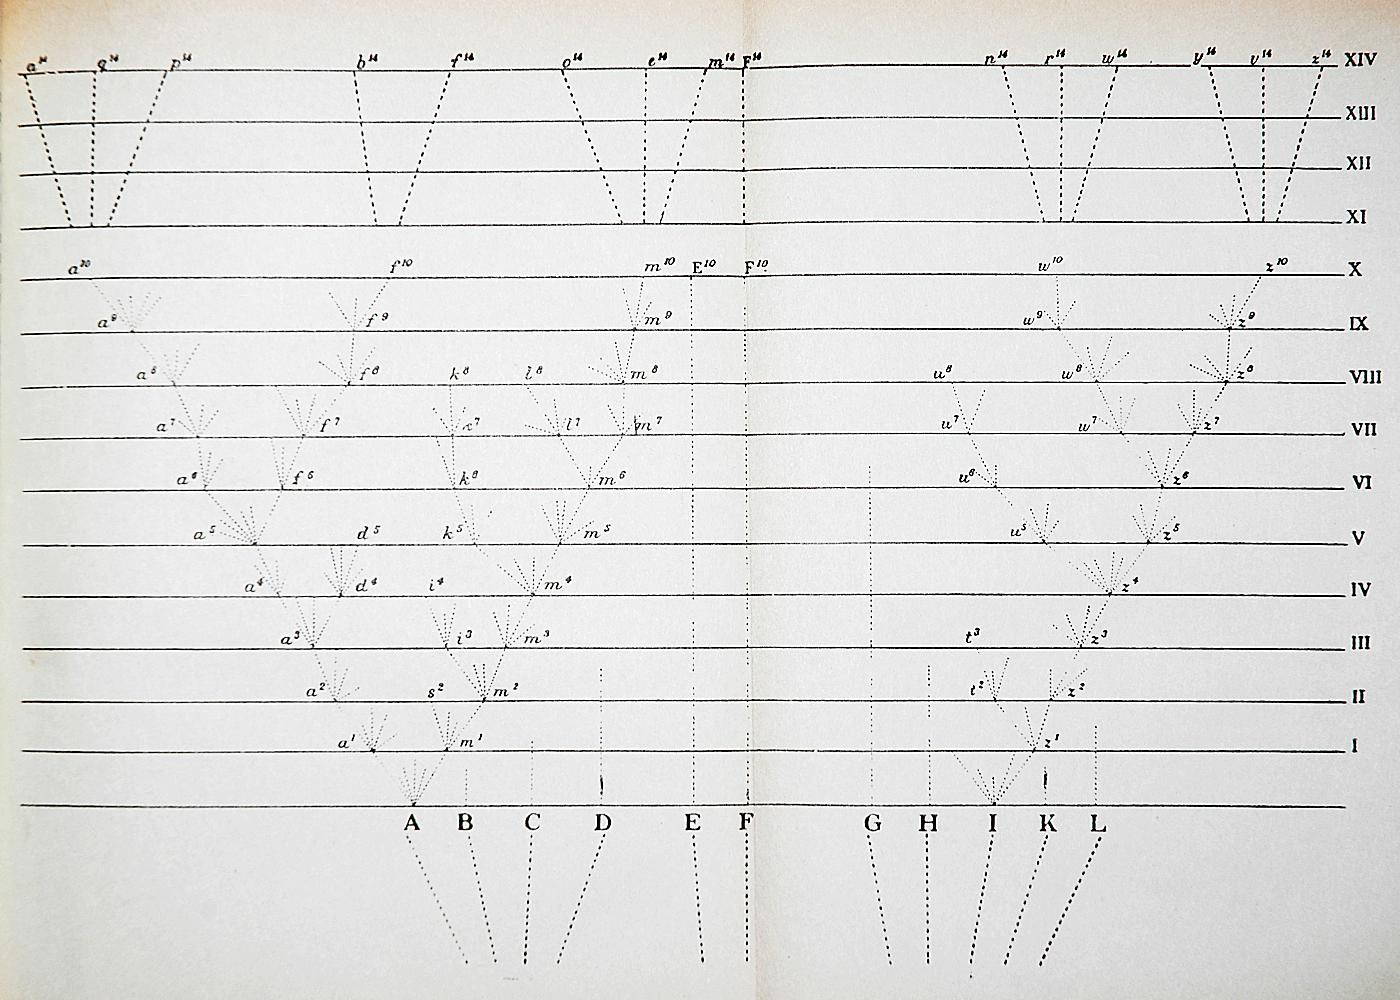
\includegraphics[width=.5\columnwidth]{./fig/introduction/Darwin_divergence.jpg}
% \caption[Charles Darwin's Evolutionary Tree]{The only figure in Darwin's \emph{On the Origin of Species}. Darwin argued for descent with modification and natural selection as the driving processes underscoring evolution. In this figure, Darwin sketched his idea for how diverging species would result in a tree structure. Reproduced from \cite{Darwin:1859uh}.}
% \label{fig:darwin_origin}
% \end{figure}

\begin{figure}
\centering
\includegraphics[]{./fig/introduction/darwin2.pdf}
\caption[Charles Darwin and the Evolutionary Tree]{(A) Charles Darwin in 1881. Photograph by Herbert Rose Barraud. (B) An sketch from Darwin's notebooks (circa 1837) showing an early conception of the evoutionary tree. (C) The only figure in Darwin's \emph{On the Origin of Species}. In \emph{The Origin}, Darwin argued for descent with modification and natural selection as the driving processes underscoring evolution. In this figure, Darwin illustarted his idea for how diverging species would result in a tree structure. Reproduced from \cite{Darwin:1859uh}.}
\label{fig:darwin_origin}
\end{figure}

\section{Molecular Evolution and the Tree Paradigm}

The combination of Darwin's theory of natural selection with Mendelian genetics led to the \emph{modern evolutionary synthesis}, outlined in the first half of the twentieth century in pioneering works by Ronald Fisher, Sewall Wright, JBS Haldane, and others.\footnote{See \cite{Huxley:1942} and \cite{Gould:2002ts} for comprehensive historical reviews.}
The modern synthesis was based largely on an analysis of distributions of allele frequencies in distinct populations, the purview of classical population genetics.
The field was placed on a molecular foundation with Watson and Crick's discovery of the DNA double-helix in 1953 \cite{Watson:1953wm}.
These developments led to the establishment of \emph{molecular evolution}, the analysis of how processes such as mutation, drift, and recombination act to induce changes in populations and species.

The information underlying an organism's form and function is encoded in its genome, the complete sequence of DNA (or RNA) contained in each cell.
The genome can be represented as a string of nucleotides, indexed by position.
Embedded within the genome are regions defining the genes which code for functional proteins, as well as non-coding regions which have as-yet unknown function.\footnote{In humans, only 1.5\% of the genome is protein-coding, the rest largely non-functional \cite{Lander:2001hk}. Up to 5-8\% of the human genome is believed to consist of endogenous retroviruses, dead viruses which have integrated their genome into the human genome \cite{Belshaw:2004gw}.}
When an organism reproduces, either sexually or asexually, a complete copy of this genomic information is passed to the offspring.
Because the molecular mechanisms that control this copying are not exact, errors in replication are introduced.
These errors can take the form of single point mutations (or single nucleotide polymorphisms, SNPs), small insertions and deletions of a few nucleotides (indels), or larger effects including copy number variations (CNVs) and chromosomal duplications.\footnote{Mutation rate vary across species: in humans, $10^{-8}$ per site per generation \cite{Nachman:2000um}; in bacteria and unicellular eukaryotes, between $10^{-9}$ and $10^{-10}$ per site per generation; in DNA viruses, between $10^{-6}$ and $10^{-8}$ per site per generation \cite{Drake:1998kv}.}
Under the neutral theory of evolution, the majority of these errors will have very little impact, either positive or negative, on the descendant organism.
A small fraction of mutations will result in an appreciable fitness difference compared to other organisms, and it is on these organisms that natural selection will act.

While molecular biology has largely focused on the biochemical and biophysical mechanisms underlying these processes, \emph{molecular phylogenetics} has focused on the comparative analysis of macromolecular sequences to infer genealogical and evolutionary relationships.
Molecular phylogenetics began with Emile Zuckerkandl and Linus Pauling's recognition in the early 1960's that the information encoded in a set of molecular sequences could itself be used as a document of evolutionary history \cite{Zuckerkandl:1962,Zuckerkandl:1965wi}.
It became clear that given two sequenced organisms, counting the differences between their respective sequences could be used as a quantitative measure of the amount of evolutionary divergence between the two organisms.
If one has a larger set of sequenced organisms, computing the complete set of pairwise distances yields a \emph{distance matrix}.
From the distance matrix, one can then attempt to associate a tree to the data such that pairwise distances along the tree are close to the measured pairwise distances from the sequences.
Walter Fitch and Emanuel Margoliash popularized this approach by constructing a weighted least squares approach to fitting phylogenetic trees from distances \cite{Fitch:1967we}.
Since that time, the development of numerical approaches for inferring evolutionary relationships has evolved into a mature discipline and the use of molecular sequence data to infer phylogeny has become a standard practice across a wide range of biology and ecology.
While other approaches to tree inference have been developed, including parsimony, maximum likelihood (ML), and Bayesian methods, we will focus on distance matrix methods because of their close relationship to the topological ideas we employ.

One important early result from molecular phylogenetics was Carl Woese's organization of bacteria, eukarya, and archaea into the three domains of life \cite{Woese:1977vd}.
Prior to Woese, there were two recognized domains of life: prokaryotes, single-celled organisms lacking a nucleus, and eukaryotes, multi-celled organisms with an enveloped nucleus.
Using 16S subunit ribosomal RNA sequencing, Woese discovered that the prokaryotic domain actually split into two evolutionarily distinct groups.
One of these, which he termed \emph{archaebacteria} was more closely related to eukaryotes than were there the rest of the prokaryotes.
This led to the three-domain system of life (Figure \ref{fig:woese_tree}).

\begin{figure}
\centering
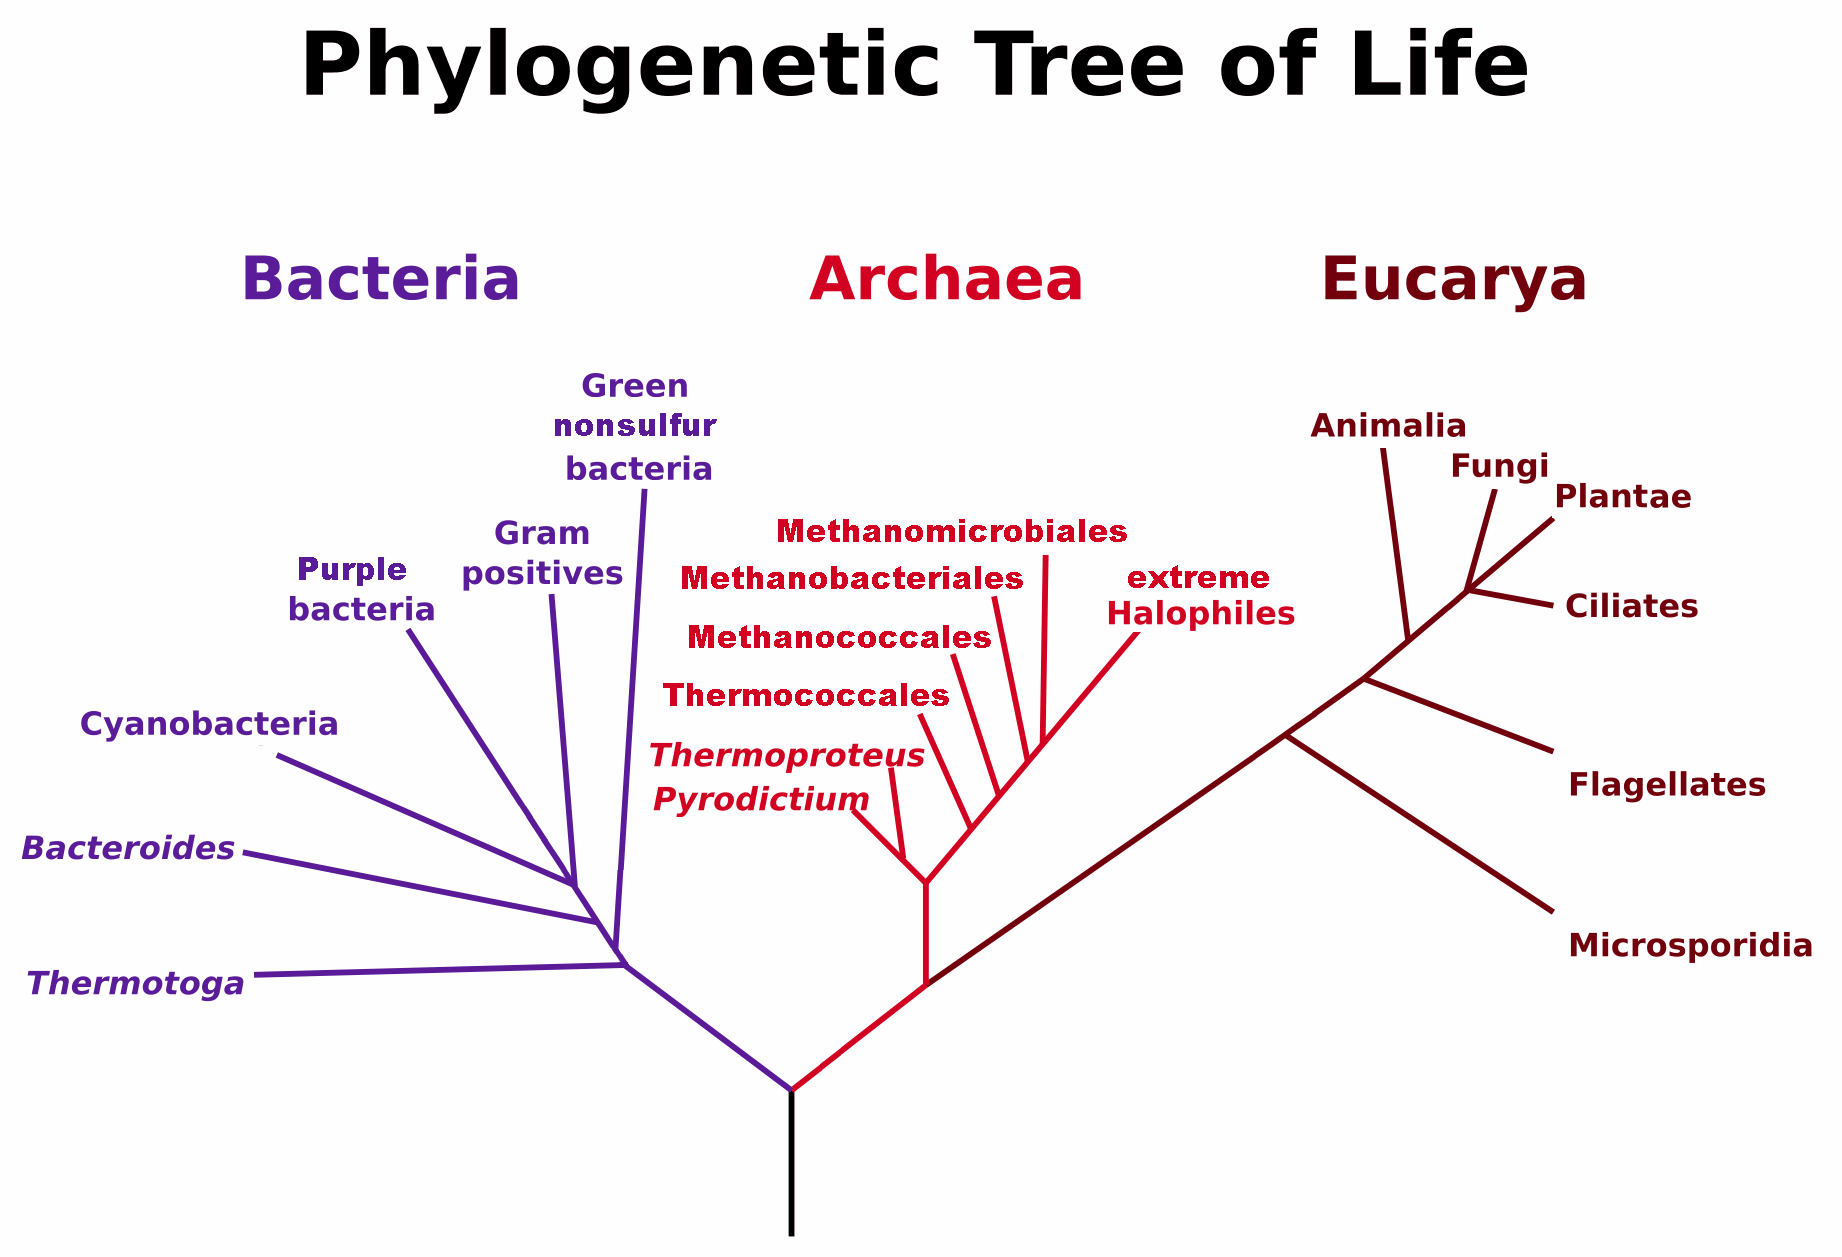
\includegraphics[width=.7\columnwidth]{./fig/introduction/woese_tree.png}
\caption[Carl Woese's Three Domain Tree of Life]{Carl Woese's three domain tree of life. Using 16S subunit ribosomal RNA, Carl Woese identified archaea as a distinct phylogenetic domain. Previously, based on morphological similarity (specifically, unicellular and lacking a nucleus), archaea had been grouped with bacteria. This result was an early success for molecular phylogenetics and the use of conserved gene segments for molecular classification. Figure adapted from \cite{Woese:1990uc}.}
\label{fig:woese_tree}
\end{figure}

This work had several important consequences.
First, it established the use of molecular data to inform about large-scale patterns of evolutionary history.
Using only morphological data had led to an inconsistent classification of archaea.
Second, it positioned 16S rRNA profiling as the primary source of data for use in comparative genomics.
The use of this genomic region was justified on the basis of being one of the few universal gene segments that is conserved across all species.
Constructing a universal tree is predicated on there being orthologous genes, i.e. shared genes related through speciation events, that can provide a common foundation for comparative study.
Finally, it solidified the tree paradigm as an organizing principle for relating extant species.
Even though reticulate processes had been known since the early twentieth century\footnote{Beginning with Frederick Griffith's experiments in 1928 showing that non-virulent strains of \emph{Streptococcus pneumoniae} could acquire virulence factors by being exposed to dead virulent strains.}, the idea that evolutionary relationships should be described by a bifurcating tree had been paramount since Darwin. 
Reticulate processes were either ignored completely, or expected to occur at such low frequencies that they need not be considered.

\section{Reticulate Processes and the Universal Tree}

Despite the significant impact of Woese's observation, there remained a subtle difficulty, which Woese himself would come to contemplate in later work \cite{Woese:2004ba,Goldenfeld:2007im}.
Woese's phylogeny was based on only 1,500 nucleotides in the ribosomal RNA, less than 1\% of the total length of a typical bacterial genome (see \cite{Dagan:2006up}).
Even more striking, this accounts for less than 0.00005\% of the human genome.
While recent work has developed approaches for constructing reference trees from larger gene sets \cite{Ciccarelli:2006gw}, the fact remains that the vast majority of genomic information is \emph{not} incorporated into the tree.

The reason for this situation is twofold.
First, not all genes are shared universally across all species.
In constructing a phylogenetic tree using sequence data, only genes that are present across all species are informative.
Second, even among universal genes, the presence of reticulate evolutionary processes will confound systematic analysis.
The model of a bifurcating tree will be consistent only if all loci share the same pattern of bifurcation.
When organisms can exchange genetic material by means other than direct reproduction, the ancestral relationships between organisms will depend on which genomic regions are used.
If two different genomic regions were analyzed, two different tree topologies may be generated, yielding conflicting phylogenetic information.
It remains an open question how to best construct a consistent evolutionary history from conflicting phylogenetic signals\footnote{There exists a cottage industry of methods for aggregating conflicting \emph{gene trees} into a consensus \emph{species tree}, see \cite{Maddison:1997ew}.}

Historically, reticulate processes were believed to occur at such a low frequency that they could be safely ignored when considering evolutionary relationships.
However, new genomic data has shown that, particularly in microorganisms such as bacteria and archaea, reticulate processes are much more prevalent than originally expected \cite{Ochman:2000dr}.
Incompatibilities in the tree paradigm now appear as the rule, not the exception, which has led to calls for new representations of evolutionary relationships \cite{Doolittle:1999,Doolittle:2006}.
Many have argued that, in light of new genomic evidence, the very notion of a universal tree of life must be discarded \cite{Koonin:2008bt,Koonin:2008tj}.
This point has been argued most strongly by Ford Doolittle of Dalhousie University.
In Figure~\ref{fig:doolittle_tree}, we see Doolittle's simplified representation of Tree of Life as it stands today, including only two of the most well-known reticulate events: the acquisition of mitochondria and chloroplasts from bacterial ancestors.
We also see his representation of the Tree of Life as it would stand if additional large-scale reticulations were reflected -- no longer is it clear that the tree is an appropriate metaphor.

\begin{figure}
\centering
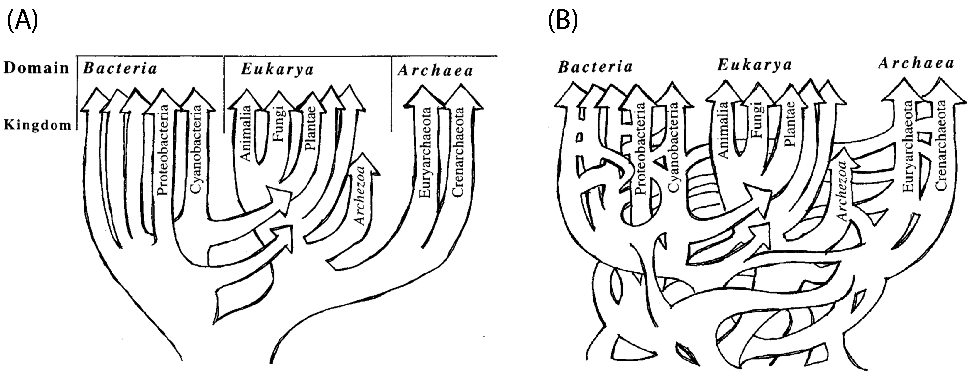
\includegraphics[]{./fig/introduction/doolittle_trees.pdf}
\caption[Ford Doolittle's Reticulate Tree of Life]{(A) W Ford Doolittle's representation of the consensus universal tree of life. Only the most well known reticulations are reflected: the endosymbiosis of mitochondria and chloroplasts. (B) Doolittle's speculative representation of the universal tree of life after accounting for reticulate evolution. While the three domains of life are still recognizable, patterns of divergence no longer follow a strictly treelike model. (From \emph{Science}, vol. 284, issue 5423, page 2127. Reprinted with permission from AAAS.)}
\label{fig:doolittle_tree}
\end{figure}

Finally, reticulate evolutionary processes are of more than just historical interest for evolutionary studies, but play a substantial role in human health and disease.
In HIV, frequent homologous recombination confounds our understanding of the epidemic's early and present history \cite{Burke:1997ep}.
In influenza, segmental gene reassortments lead to antigenic novelty and the emergence of epidemics \cite{Nelson:2007bc}.
In several pathogenic bacteria, including \emph{E. coli} and \emph{S. aureus}, horizontal gene transfer has been responsible for the spread of antibiotic resistance genes \cite{Alekshun:2007bq,Davies:2010dv}.
For example, the 2011 German \emph{E. coli} outbreak was caused by a strain of \emph{E. coli} that had acquired the ability to produce Shiga toxin \cite{Rohde:2011ju}.

\section{Evolution as a Topological Space}

We propose the use of new computational techniques, borrowed from the field of applied topology, to capture and represent complex patterns of reticulate evolution.

Topology as a mathematical field is concerned with properties of spaces that are invariant under continuous deformation.
Such properties can include, for example, connectedness and the presence of holes.
Two objects are considered topologically equivalent if they can be deformed into one another without introducing any cuts or tears.
As a paradigmatic example, consider the coffee mug and the donut (Figure~\ref{intro:fig:coffeemug_to_donut}).
While seemingly different, it is not difficult to see that both objects consist of a single connected component that is wrapped around a single hole.
Were the objects smoothly pliable they could be freely deformed into one another.
Topologically, the two objects are equivalent.\footnote{The two objects are topologically equivalent to a solid torus, which is represented as $D^2\times S^1$, a solid two-dimensional disk wrapping around a circle.}

\begin{figure}[t]
\centering
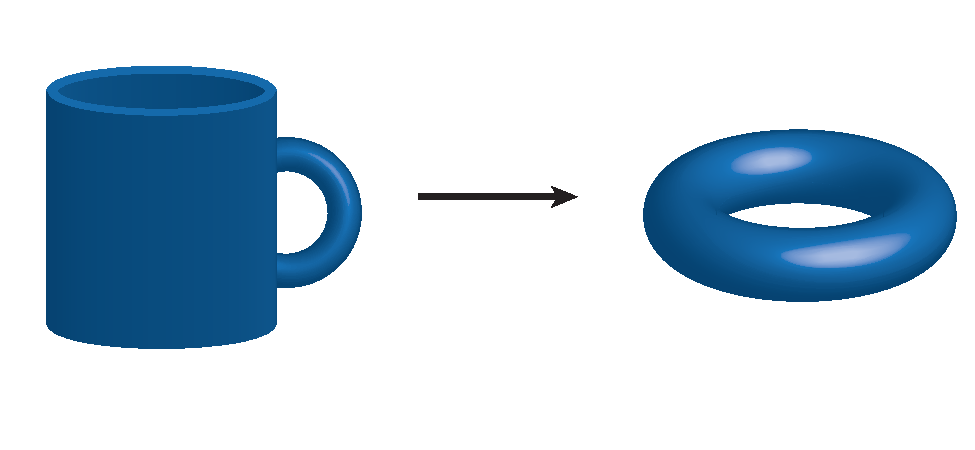
\includegraphics[width=\columnwidth]{./fig/introduction/coffeemug_to_donut.pdf}
\caption[Topological equivalence of the coffee mug and the donut]{The paradigmatic example of topological equivalence. The coffee mug can be continuously deformed into the donut and are therefore topologically equivalent. Both exhibit the topology of a solid torus ($D^2\times S^1$).}
\label{intro:fig:coffeemug_to_donut}
\end{figure}

Algebraic topology quantifies our intuitive notions of shape using algebraic structures to represent different invariants of a space.
For our purposes, the most relevant invariants will be the \emph{Betti numbers}.
We give a more complete characterization of Betti numbers in Chapter~\ref{ch:background}, but the intuition is as follows.
The Betti numbers are a collection of integers indexed by an integer $n$ describing the connectivity of a space at different dimensions.
First, we can think of $\betti_0$ as representing the number of connected components, or clusters, in our space.
Next, we can think of $\betti_1$ as representing the number of one-dimensional loops in our space.
Equivalently, this is the number of cuts needed to transform the space into something simply connected.\footnote{In a simply connected space, any path between two points can be deformed into any other such path.}
Higher Betti numbers, $\betti_n$ for $n>1$ will correspond to higher dimensional holes.
In our coffee mug example, because both objects have the same Betti numbers ($\betti_0=1$, $\betti_1=1$, and $\betti_n=0$ for $n>1$), they are considered topologically equivalent.
Our goal in this work will be to adopt a similar perspective and characterize evolutionary spaces as topological spaces using their Betti numbers.

To give a simple example, consider Figure~\ref{intro:fig:simple_tree_example}.
The example presents two possible scenarios describing the evolutionary relationships of three species, labeled $a$, $b$, and $c$.
For each scenario, moving vertically up the object corresponds to moving backwards in time.
Branch lengths correspond to evolutionary divergence.
Internal vertices represent extinct ancestors of the three species, up to the root of the tree, $r$, which represents the most recent common ancestor.
On the left, we have a simple tree topology relating the three species.
Considering the shape of the tree, there is a single connected component, giving $\betti_0=1$.
Further, we see that there are no loops formed by the branches, giving $\betti_1=0$.
The object is therefore considered trivially contractible, a property which will hold for all tree topologies.
On the right, we have a reticulate topology relating the three species.
We can envision species $b$ as being the reticulate offspring of parents ancestral to species $a$ and $c$.
That is, species $b$ carries unique genetic material from both species $a$ and species $c$.
To account for this, two branches merge into the vertex that is directly ancestral to $b$.
Considering the shape, there is again a single connected component, giving $\betti_0=1$.
However, because of the reticulate event mixing material from $a$ and $c$, there is now a loop formed in the topology, giving $\betti_1=1$
The object is no longer treelike and is characterized by a more complex topology.
The Betti numbers capture the essential difference in the two evolutionary histories.
Finally, we note that this is a conceptual example of how reticulate processes can be captured using topology -- in practice, we do not have access to the true history, but must infer it from a finite sample.

Consider again Darwin's branching phylogeny (Figure~\ref{fig:darwin_origin}) and Doolittle's modified representation after accounting for reticulate evolution (Figure~\ref{fig:doolittle_tree}).
The two objects can be imagined to be representations of two different topological spaces.
Darwin's branching phylogeny is a tree and hence trivially contractible ($\betti_n=0$ for $n>0$).
In contrast, Doolittle's construction has a much more complex topology, with loops being formed where reticulate events have occurred.
The object will be characterized by nonvanishing Betti numbers, the magnitude of which will be associated with the amount of reticulation that has occurred.
The remainder of this thesis focuses on expanding this idea and applying it to real data sets with the goal of measuring the prevalence and scale of reticulate evolutionary events.
Our aim will be to characterize reticulate exchange of genetic material by the parental sequences involved in the exchange, by the amount and identity of material exchanged (i.e., the genes or loci involved), and the frequency with which similar exchanges occur.
Several important questions will be dealt with, such as how to construct topological spaces from finitely sampled sequence data, how to make comparisons among gene sets, and how to make statistical statements about reticulate events.
We will address these questions by developing new techniques to construct and extract topological and statistical information from evolutionary data.
In doing so, we provide a fuller understanding of evolutionary relationships than possible with current phylogenetic methods.

\begin{figure}
\centering
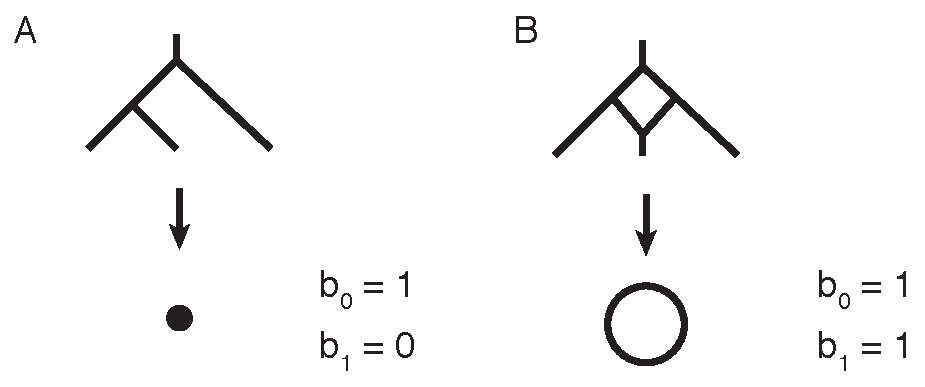
\includegraphics[width=.8\columnwidth]{./fig/introduction/simple_tree_example.pdf}
\caption[Treelike and reticulate phylogenies]{(A) A simple treelike phylogeny is contractible to a point. (B) A reticulate phylogeny that is equivalent to a circle and not contractible without a cut. The two spaces are not topologically equivalent and can be distinguished by their Betti numbers.}
\label{intro:fig:simple_tree_example}
\end{figure}

\section{Thesis Organization}

The remainder of this thesis is organized as follows.

In Chapter \ref{ch:background} we present background material on the topics discussed in this thesis.
This discussion is chiefly structured into two pieces: (1) background on phylogenetics and population genetics, and (2) background on the methods we use from TDA.

In Part \ref{part:theory}, we develop two complementary approaches for analyzing sequence data using TDA.
In Chapter \ref{ch:complex_construction}, we propose methods of constructing topological spaces that generalize standard constructions but are suited to the particular requirements of phylogenetic applications.
We draw on previous work in phylogenetic networks and use homology to provide a quantitative assessment of reticulate processes.
This work was published in \cite{Emmett:2015a}.
In Chapter \ref{ch:parametric_inference}, we develop methods for performing statistical inference using summary statistics computed using methods from TDA.
This is the first such use of TDA as a tool for performing parametric inference and should generalize to a wide range of application settings.
This work was published in \cite{Emmett:2014b}

In Part \ref{part:applications}, we apply our approach to several problems in evolution and genomics.
In Chapter \ref{ch:phage} we study phages, viruses of single-celled microorganisms.
We show how persistent homology recovers inconsistencies in existing morphology-based taxonomies, use a network approach to construct an alternative genome-based representation of phage relationships, and identify representative gene families conserved within phage populations.
In Chapter \ref{ch:influenza} we study influenza, a common human pathogen.
We show how persistent homology captures widespread patterns of reassortment, including nonrandom cosegregation of segments and barriers to subtype mixing.
In contrast to traditional influenza studies, which focus on the phylogenetic branching patterns of only the two surface-marker proteins, we use Mapper combined with whole-genome data to represent influenza molecular relationships.
We show unexpected relationships between divergent influenza subtypes.
This work draws from results in \cite{Chan:2013} and \cite{Emmett:2014b}.
In Chapter \ref{ch:pathogens} we study pathogenic bacteria.
We use two sources of data to measure rates of reticulation in both the core genome and the mobile genome across a range of species.
Mapper is used to represent the population of \emph{S. aureus} and analyze the spread of antibiotic resistance genes.
The potential for the spreading of antibiotic resistance in the human microbiome is investigated.
This work was published in \cite{Emmett:2014a}
%In Chapter \ref{ch:hic} we analyze high-throughput chromatin interaction data to explore patterns of chromatin folding in the nucleus in simulated, prokaryotic, and human datasets.

Finally, in Chapter \ref{ch:conclusions} we summarize these results and present future research directions.